\documentclass[a4paper]{scrreprt}
\usepackage{fancyhdr}
\pagestyle{fancy}
\usepackage[english]{babel}
\usepackage[utf8]{inputenc}
\usepackage{graphicx}
\usepackage{url}
\usepackage{textcomp}
\usepackage{amsmath}
\usepackage{lastpage}
\usepackage{pgf}
\usepackage{wrapfig}
\usepackage{fancyvrb}
\usepackage{appendix}
\usepackage{pdfpages}
\usepackage{xcolor}
\usepackage{hyperref}

\hypersetup{
    colorlinks=true,
    linkcolor=blue,
    filecolor=black,      
    urlcolor=blue,
    citecolor=black,
}

% Create header and footer
\headheight 27pt
\pagestyle{fancyplain}
\lhead{\footnotesize{Datalagring, IV1351}}
\chead{\footnotesize{Task 2}}
\rhead{}
\lfoot{}
\cfoot{\thepage\ (\pageref{LastPage})}
\rfoot{}

% Create title page
\title{Task 2, version 2}
\subtitle{Datalagring, IV1351}
\author{Adrian Jonsson Sjödin \\ adriansj@kth.se}
\date{\today} 


\begin{document}

\maketitle

\tableofcontents %Generates the TOC

\chapter{Introduction}
The purpose of task 2 was to turn the conceptual model of the Sound Good Music School database developed in task 1, into a logical model. That is a model that we can 
use when creating our database in MySQL. The creation and reasoning behind this logical model is what will be covered in this report.



\chapter{Method}
To turn our conceptual model (see fig. \ref{fig:conceptualModel}) into a logical model we mostly followed the steps laid out in the lecture about logical and physical models.

First we copied our conceptual model into the logical model and then proceeded to delete all relationships so that we where only left with the tables, and after this we 
went through each table and made sure they where 1NF and no row contained duplicated data. This resulted in some new tables. After this we specified the type for each column 
and whether or not it should allow NULL.

Then the next step was to achieve 2NF and start creating the Primary Keys and draw the relationships between the tables, and consider which Foreign Keys can be allowed 
to be NULL. Drawing the relationships resulted in some tables being deleted.

The last step was to split up some tables a bit more to try and achieve 3NF.

Having the logical model done we created the database using Astah's export to SQL function. Unfortunately you can not directly use it since it gave quite a lot of errors,
but it gave a good foundation to build upon.

Having this foundation to build upon we went through it from top to bottom while looking at the logical model to make sure everything is implemented correctly. During this process 
we did some changes to the logical model when discovering mistakes we had overlooked. 

For writing the SQl scripts that created the databases and populated it with data MySQL Workbench and DbGate was used. The logical model was created in Astah Pro. 

\begin{figure}[h]
    \begin{center}
        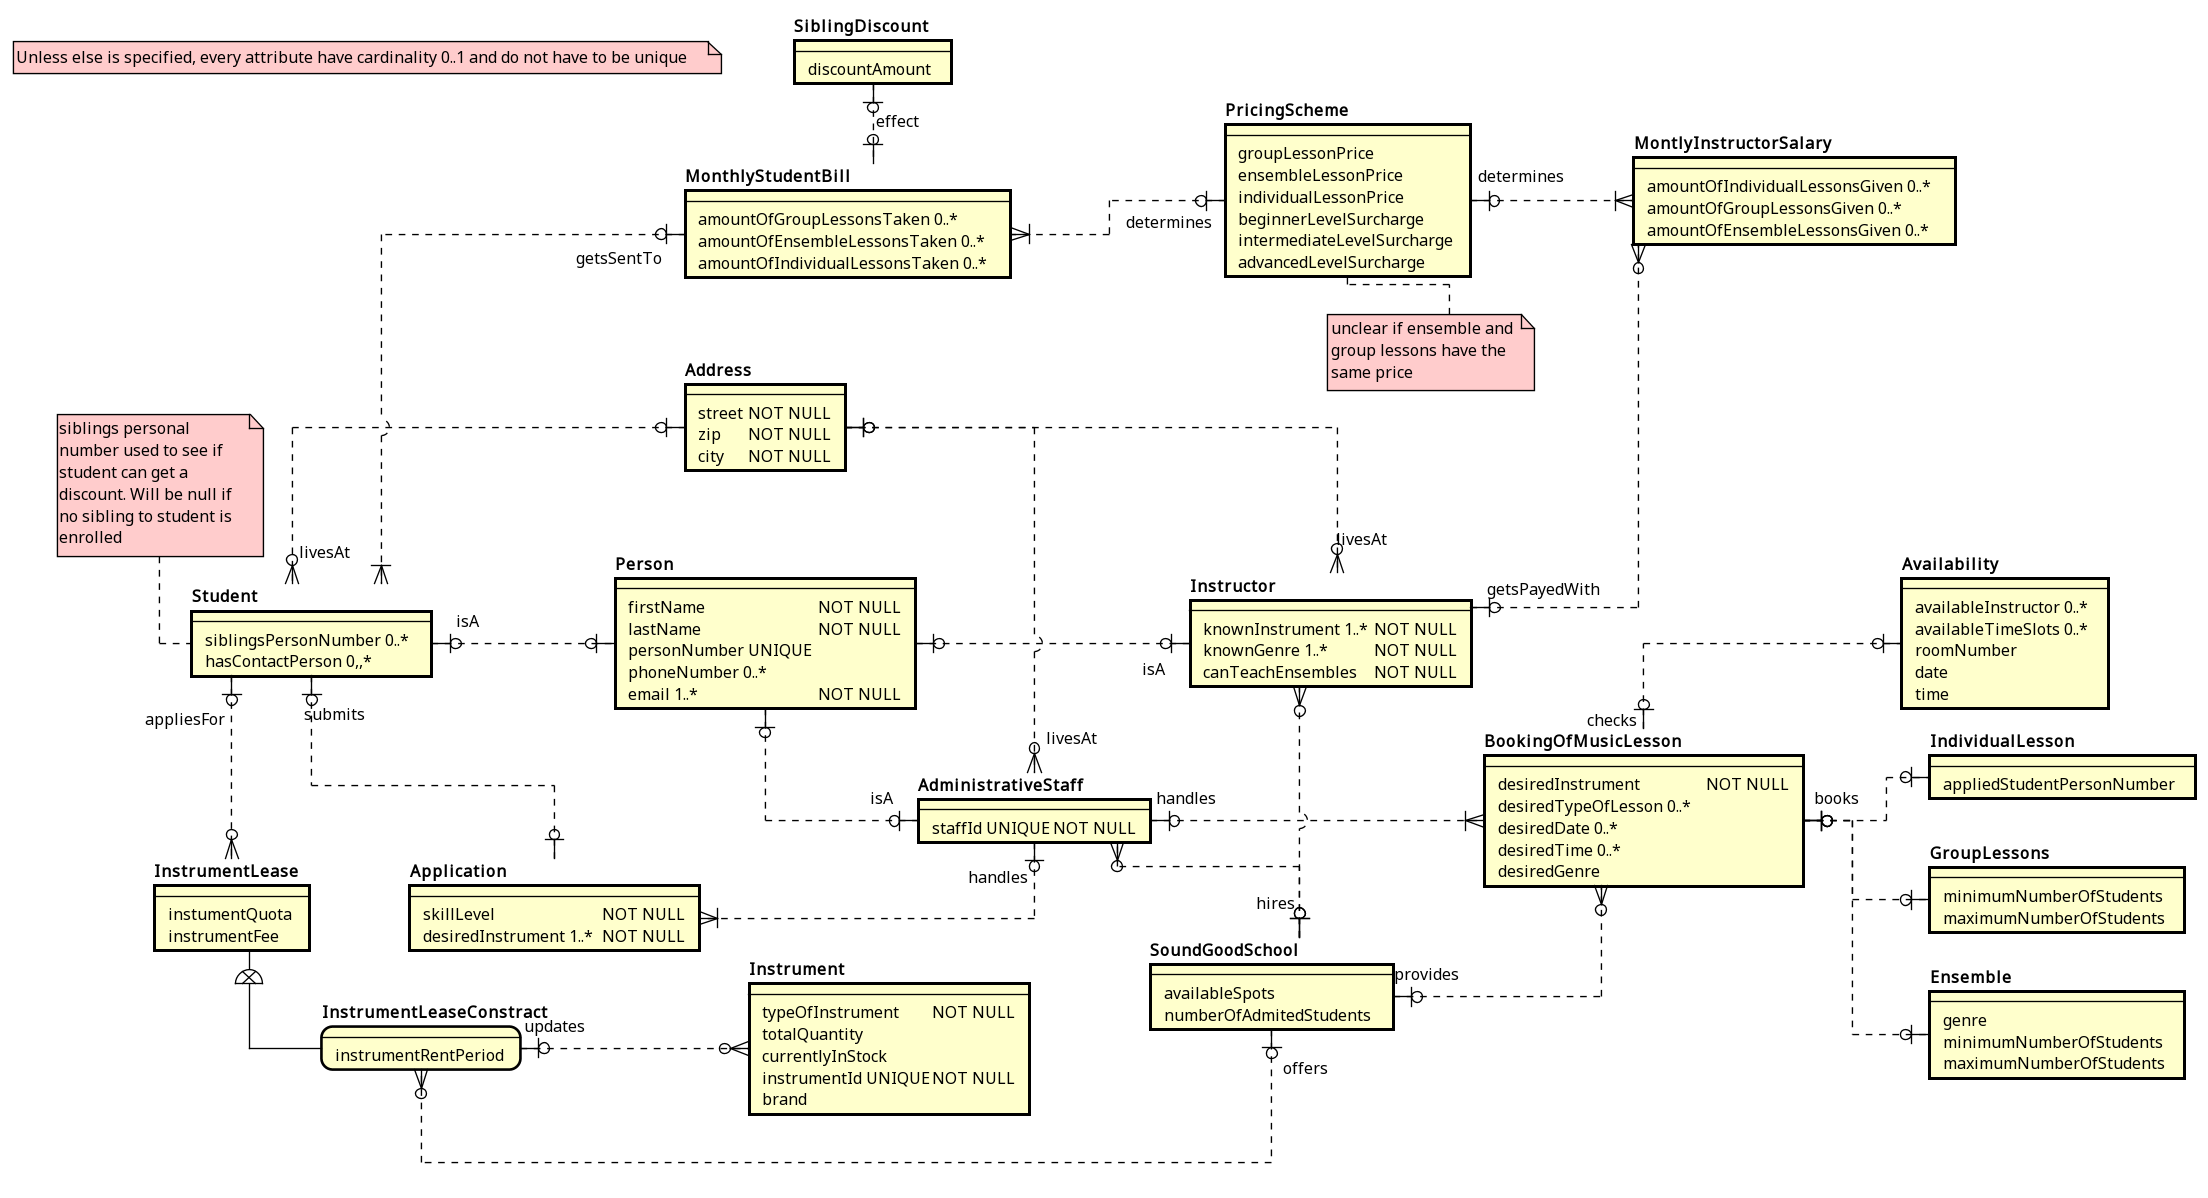
\includegraphics[width=\textwidth]{../img/conceptualModel.v1.0.1.png}
        \caption{Conceptual Model for the SoundGood music school database}
        \label{fig:conceptualModel}
    \end{center}
\end{figure} 

\chapter{Result}

\label{sec:result}
In figure \ref{fig:logicalModel} we can see the finished logical model. 
I tried to have as little duplicated data as possible which is why I decided to have a table "addresses" instead of having an address column in "person" and 
"sound\_good\_music\_school". They will instead have a Foreign Key to the address, which will keep the table smaller and save memory since we will not have multiple
rows with the same values for people living at the same address. The same reasoning is behind the "parent" and "student" table with them having a Foreign Key to "person", which we can use to retrieve their 
data. 
The most important part of the model is arguably how lessons are booked. As can be seen in figure \ref{fig:logicalModel} we have a table "music\_lesson" which contains all the available lessons. As can be seen 
in the "booking" table, a booking will have a foreign key to the corresponding music lesson and this key will also be the primary key for the corresponding type of music lesson. Furthermore we added some triggers
to the database that makes sure a student can not have two bookings on the same time and day, and to make sure that lessons that are full can not be booked.


The SQL scripts can be found here:
 \href{https://github.com/adrian-jonsson-sjoedin/IV1351-Datalagring/tree/main/project/SQL}{GitHub}.


\begin{figure}[h]
    \begin{center}
        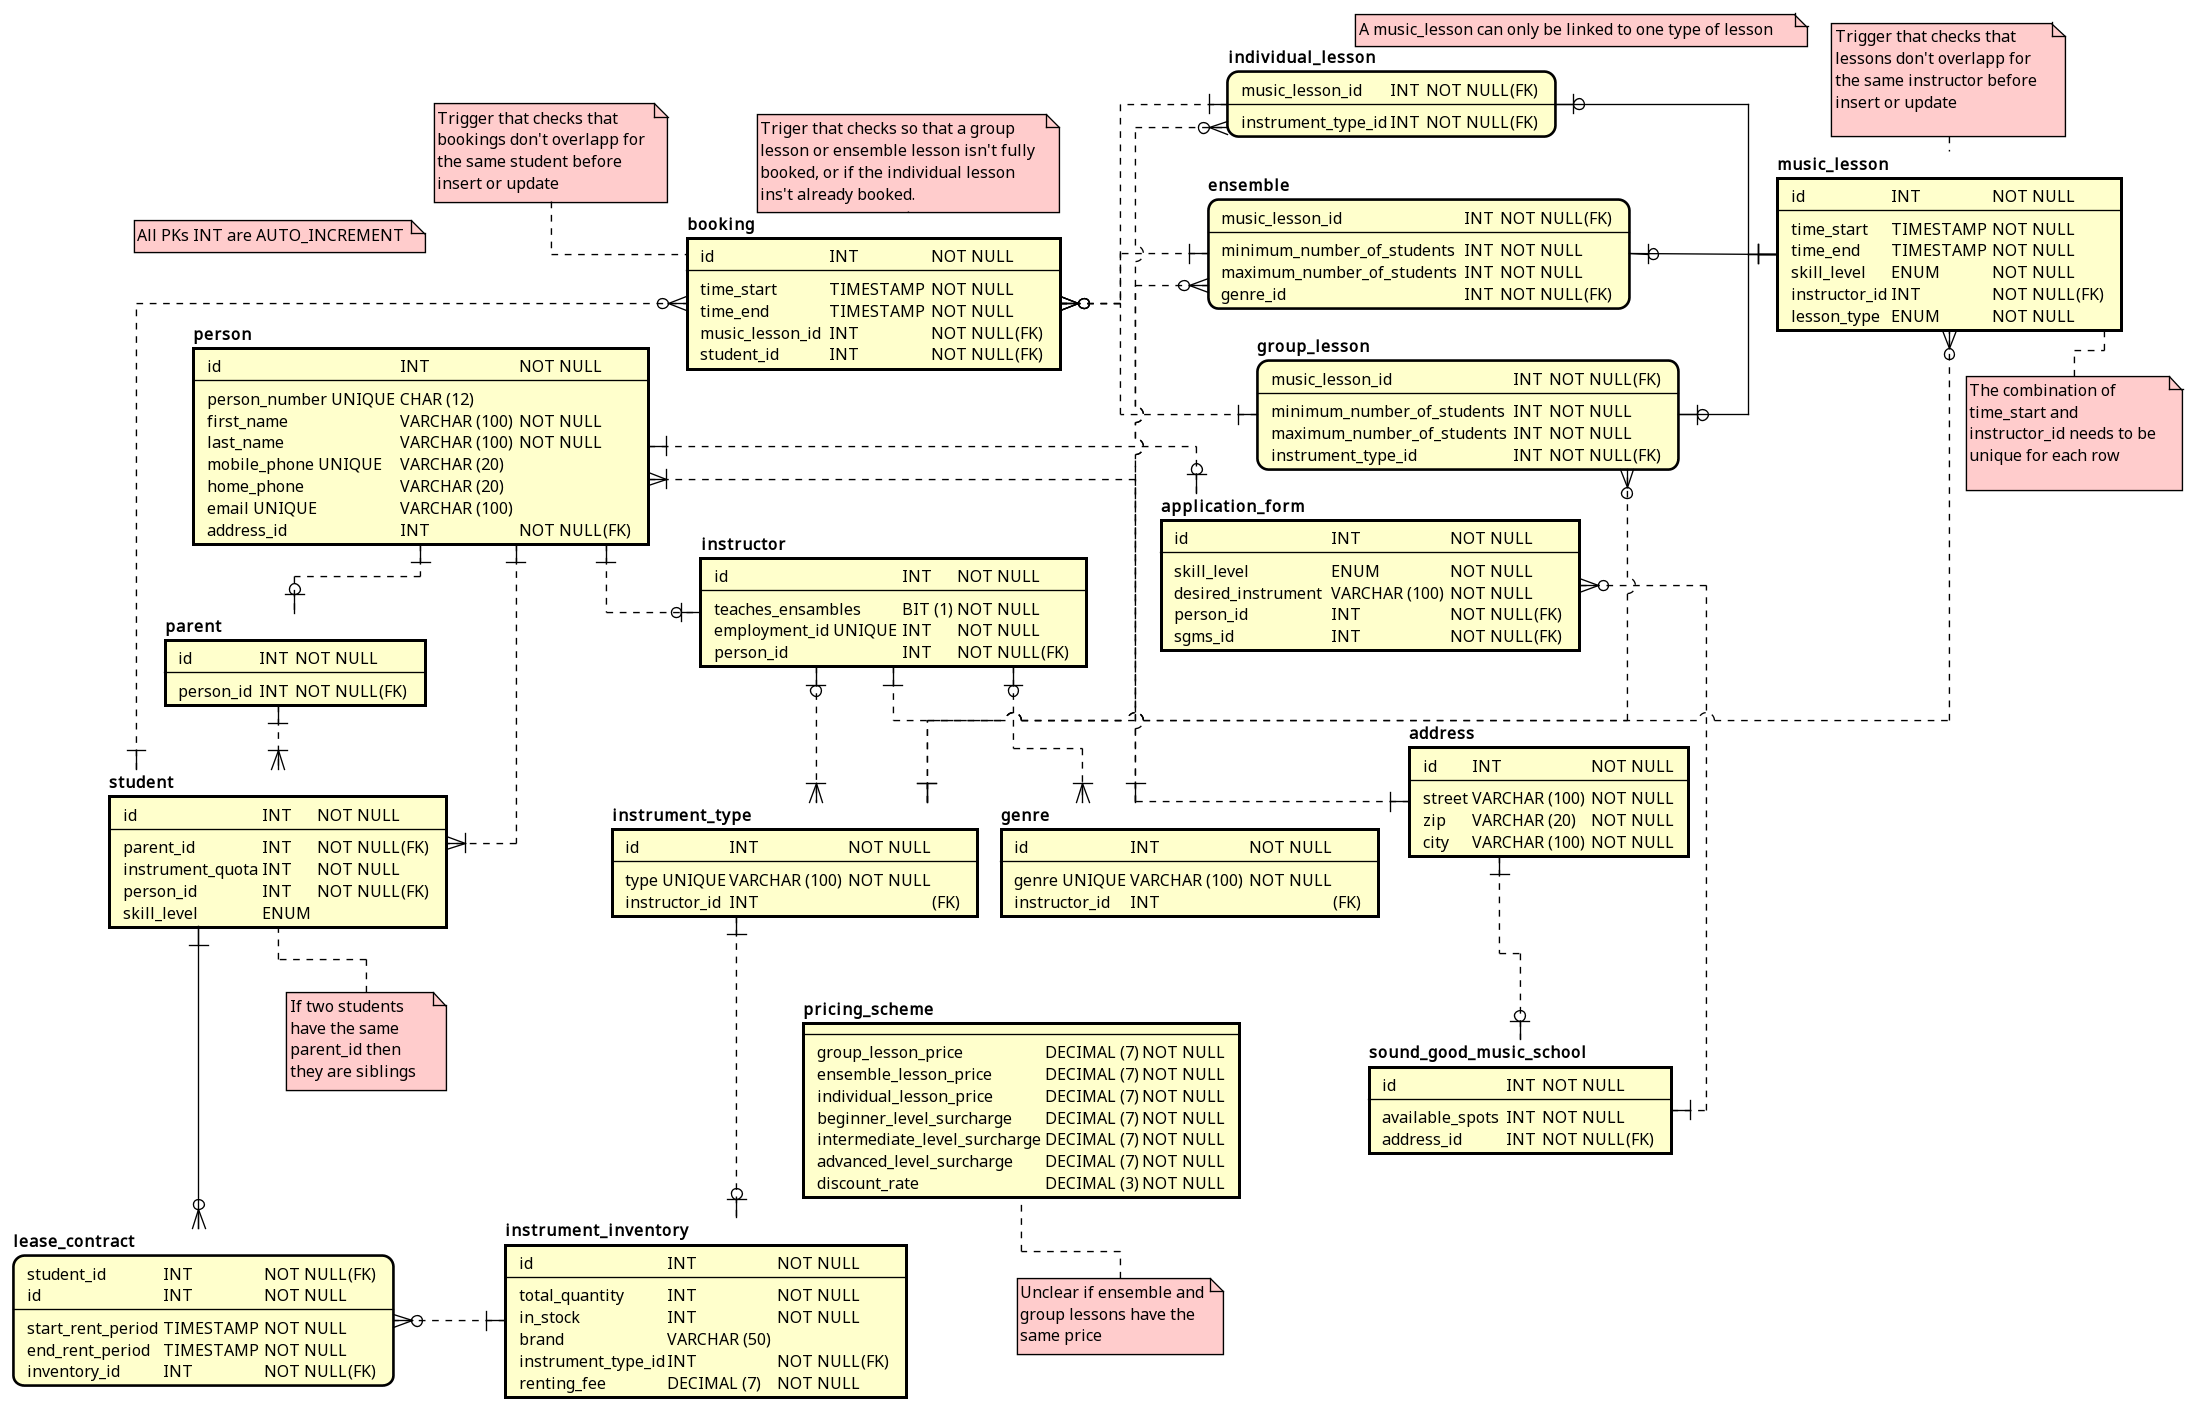
\includegraphics[width=\textwidth]{../img/LogicalModel_v3.png}
        \caption{The logical model for the SoundGood music school database}
        \label{fig:logicalModel}
    \end{center}
\end{figure}



\chapter{Discussion}
While converting the Conceptual Model into a Logical Model I noticed quite a few flaws that needed correcting. For starters I had the administrative staff in the database,
which is not a requirement since their roll was to use an application that interacts with the database. They handle the bookings and such but the task here was not to 
model a booking system but rather a database system. 

I also added a table "parent" since I realized having an attribute "hasContactPerson" is not the best way to store data about a students parents. Instead "student" now 
have a Foreign Key referencing "parent" and "parent" have a Foreign Key referencing "person". This will also help us calculate which students are siblings since they 
will have the same Foreign Key to parents. 

Another big change is how instruments and the leasing of them is handled. I moved the "instrumentQuota" into "students" and "instrumentFee" into "instrument\_inventory"
thus removing the "InstrumentLease" table seen in fig. \ref{fig:conceptualModel}. The "instrumentLeaseContract" then became the "lease\_contract" and since the same 
student can rent multiple instrument we hade the make the Primary Key a Composite Key using the Foreign Key from "students" and a Surrogate Key. So each row in this
table would represent a lease contract. For the instruments I decided against assigning each single instrument its own serial number and instead went with the approach
of just storing how many instrument of a certain type we have. This is of course something that would have to be discussed with the client, but doing it this way 
simplified the design. 

Speaking of the instrument type, we also created a new table just for that since it helped reducing the duplication of data in the "instructors" table, and we can use 
it in our "instrument\_inventory" table and the lesson tables. The reduction of duplicate data is also the reasoning behind the "genres" table.

In fig. \ref{fig:conceptualModel} we can see that we had two tables named "BookingOfMusicLesson" and "Availability", these have been removed and the tables "booking"
and "music\_lesson" have been created instead. The "booking" table is quite straightforward, it contains a foreign key to the music lesson, the time slot that they've booked and the id for the student taking it.
The foreign key "music\_lesson\_id" tells us which lesson in the "music\_lesson" table the student have booked and it is also the primary key in the three different lesson types tables. This tells us 
which lesson a student have booked and we can also see how many students have booked a group lesson or ensemble lesson by simply looking at the primary keys in for example the ensemble table and count
gow many rows there are in bookings containing that key. 

One final thing about the choice of data types and constraints. I used MySQL which is why I went for \textit{CHAR} in the once case where I knew exactly how long a 
string should be. I also used \textit{DECIMAL} since it makes it possible to define exactly how many decimals are allowed. For the constraints only NOT NULL and UNIQUE
are indicated in fig. \ref{fig:logicalModel}, but all \textit{INT}s and \textit{DECIMAL}s have the constraint that they have to be larger or equal to zero.

\end{document}
